\documentclass[xcolor=dvipsnames,pdf,11pt,handout]{beamer}
%%% Beamer options
\usetheme{inf-ufrgs}
%%% MATH
\usepackage{amsmath,amssymb,amsfonts,mathtools}
%%% Text encoding and fonts
\usepackage[utf8]{inputenc}
\usepackage[T1]{fontenc}
\usepackage{lmodern}
\usepackage{baskervald}
\usepackage[scaled=0.9]{inconsolata}
%\usepackage[LGRgreek]{mathastext}
%\setbeamercolor{math text}{fg=blue}
%\setbeamercolor{math text displayed}{fg=blue}

\setbeamercolor{math text}{fg=black}
\setbeamercolor{math text displayed}{fg=black}

\usepackage{alltt}

%%%%%%% CODE HIGHLIGHT USING MINT
\usepackage{minted}
\usemintedstyle{tango}
\setminted[haskell]
 {
    %bgcolor=yellow!50!gray!40,
    frame=single,
    framesep=0.5em,
    rulecolor=\color{lightgray},
    breaklines=true,
    linenos=true,
    numbers=left,
    numbersep=4pt,
    %resetmargins=true,
    xleftmargin=4pt
  }
\renewcommand{\theFancyVerbLine}{
  \ttfamily\textcolor[rgb]{0.6,0.6,1.0}
  %\ttfamily\textcolor[rgb]{0.9,0.9,1.0}
  {\scriptsize\arabic{FancyVerbLine}}}
\newminted[haskell]{haskell}{}

%%%% Require packages
\usepackage[all,pdf,cmtip]{xy}
\usepackage{tikz,tikz-qtree,multicol,ebproof}
\tikzset{small/.style={level distance=20pt,sibling distance=1pt}}
\tikzset{smaller/.style={level distance=20pt,sibling distance=-3pt}}

\newcommand{\dw}[2]{#1\(\sb{#2}\)}

\newcommand{\web}[1]{\url{#1}}


%%% EASY ENUMERATIONS
\newcommand{\bi}{\begin{itemize}}
\newcommand{\ei}{\end{itemize}}
\newcommand{\be}{\begin{enumerate}}
\newcommand{\ee}{\end{enumerate}}
\newcommand{\bd}{\begin{description}}
\newcommand{\ed}{\end{description}}
\newcommand{\tm}{\item}

%%% THEOREMS, DEFINITIONS, ETC... 
\newcommand{\defn}{\textcolor{blue}{\textbf{\textrm{Definition:\ }}}}
\newcommand{\thm}{\textcolor{OliveGreen}{\textbf{\textrm{Theorem:\ }}}}
\newcommand{\lem}{\textcolor{OliveGreen!50!red}{\textbf{\textrm{Lemma:\ }}}}
\newcommand{\crlr}{\textcolor{green!50!orange!80!black}{\textbf{\textrm{Corolary:\ }}}}
\newcommand{\prf}{\textcolor{Red}{\textbf{\textrm{Proof:\ }}}}
\newcommand{\exmp}{\textcolor{WildStrawberry}{\textbf{\textrm{Example:\ }}}}
\newcommand{\rmk}{\textcolor{Purple}{\textbf{\textrm{Remark:\ }}}}
\newcommand{\excs}{\textcolor{Brown}{\textbf{\textrm{Exercise:\ }}}}
\newcommand{\qstn}{\textcolor{WildStrawberry!90!black}{\textbf{\textrm{Question:\ }}}}
\newcommand{\ansr}{\textcolor{violet}{\textbf{\textrm{Answer:\ }}}}
\newcommand{\notn}{\textcolor{gray!50!black}{\textbf{\textrm{Notation:\ }}}}

\newcommand{\pp}{\pause}
\newcommand{\Red}{\color{red}}
\newcommand{\Blue}{\color{blue}}
\newcommand{\Black}{\color{black}}
\newcommand{\Maroon}{\color{Maroon}}
\newcommand{\NavyBlue}{\color{NavyBlue}}
\newcommand{\RedOrange}{\color{RedOrange}}
\newcommand{\OliveGreen}{\color{OliveGreen}}

\newcommand{\rulesequence}{$p_0,\ldots,p_{n-1},p_n$}

%%% AUTOMATIC TABLE OF CONTENTS
\renewcommand{\contentstitle}{Outline}  
\AtBeginSection[] 
{
  \begin{frame}
    \frametitle{\contentstitle}
    %\footnotesize
    %\begin{multicols}{2}
    \tableofcontents[currentsection]
    %\end{multicols}
  \end{frame}
}

%%%%%%%%%%%%%%%%%%%%%%%%%%%%%%%%%%%%%%%%%%%%%%%%%%%%%%%%%%%%%%%%%
\title     {Verigraph: a system for specification and analysis of graph grammars}
\subtitle  {}
\author    {}
\institute {\inftitle} 
\date      {}
\renewcommand{\contentstitle}{Content}  
%%%%%%%%%%%%%%%%%%%%%%%%%%%%%%%%%%%%%%%%%%%%%%%%%%%%%%%%%%%%%%%%%

\begin{document}

\titlepageVerites

%%%%%%%%%%%%%%%%%%%%%%%%%%%%%%%%%%%%%%%%
\begin{frame}
 \frametitle{\contentstitle}
 %\footnotesize
 %\begin{multicols}{2}
 \tableofcontents
 %\end{multicols}
\end{frame}
%%%%%%%%%%%%%%%%%%%%%%%%%%%%%%%%%%%%%%%%

\section{High-Level Replacement}

%%%%%%%%%%%%%%%%%%%%%%%%
\begin{frame}[fragile]{High-Level Replacement}{}

\bi
\tm Generalizes graph transformation
\tm Assumes adhesive category
  \bi
  \tm Pushouts along monomorphisms
  \tm Pullbacks
  \tm Pushouts along monomorphisms are Van Kampen squares
  \ei
\ei

\end{frame}
%%%%%%%%%%%%%%%%%%%%%%%%

%%%%%%%%%%%%%%%%%%%%%%%%
\begin{frame}[fragile]{High-Level Replacement}{}

\bi
\tm A \textbf{production} $\rho = \langle l, r \rangle$ is a monomorphic span:
\centerline{
\vspace{.25cm}
\xymatrix{
L & K\ar@{>->}@/1pc/[l]_>>{l}\ar@{>->}@/1pc/[r]^>>{r} & R
}}
\vspace{.75cm}

\tm Given a production $\rho = \langle l, r \rangle$ and a match $m$, a \textbf{transformation} is given by a double-pushout diagram:
\centerline{
\vspace{.25cm}
\xymatrix{
L\ar[d]_{m} & K\ar[d]\ar@{>->}@/1pc/[l]_>>{l}\ar@{>->}@/1pc/[r]^>>{r} & R\ar[d] \\
G\ar@{}[ur]|<<{\urcorner} & D\ar@{>->}@/1pc/[l]\ar@{>->}@/1pc/[r] & H\ar@{}[ul]|<<{\ulcorner}& 
}}

\ei

\end{frame}
%%%%%%%%%%%%%%%%%%%%%%%%

%%%%%%%%%%%%%%%%%%%%%%%%
\begin{frame}[fragile]{HLR in Haskell}{}

\bi
\tm Goal: generic algorithms with respect to the category
\tm Solution: type classes
\ei

\end{frame}
%%%%%%%%%%%%%%%%%%%%%%%%

%%%%%%%%%%%%%%%%%%%%%%%%
\begin{frame}[fragile]{Type Class: Morphism}{}

\color{blue}
\begin{haskell}
class (Eq m) => Morphism m where
    type Obj m :: *
    compose  :: m -> m -> m
    domain   :: m -> Obj m
    codomain :: m -> Obj m
    id       :: Obj m -> m
    monomorphism :: m -> Bool
    epimorphism :: m -> Bool
    isomorphism :: m -> Bool
\end{haskell}
\color{black}

\bi
\tm Class for morphisms of a category
\tm Note: full subcategory of finite objects
\ei

\end{frame}
%%%%%%%%%%%%%%%%%%%%%%%%

%%%%%%%%%%%%%%%%%%%%%%%%
\begin{frame}[fragile]{Type Class: AdhesiveHLR}{}

\color{blue}
\begin{haskell}
class (Morphism m) => AdhesiveHLR m where
  -- Assumes one of the morphisms is mono
  po :: m -> m -> (m, m)
  
  hasPoc :: m -> m -> Bool
  
  -- Assumes a pushout complement exists
  poc :: m -> m -> (m, m)
  
  -- Assumes both morphisms are mono
  injectivePullback :: m -> m -> (m, m)
\end{haskell}
\color{black}

\bi
\tm Class for morphisms of an adhesive category
\tm Pullback restricted to monomorphisms for performance
\ei

\end{frame}
%%%%%%%%%%%%%%%%%%%%%%%%

%%%%%%%%%%%%%%%%%%%%%%%%
\begin{frame}[fragile]{Data Type: Production}{}

\color{blue}
\begin{haskell}
data Production m = Production
  { left :: m   -- ^ The morphism /K -> L/ of a production
  , right :: m  -- ^ The morphism /K -> R/ of a production
  }
  deriving (Show, Read)
\end{haskell}
\color{black}

\vspace{1cm}

\centerline{
\xymatrix{
L & & K\ar@{>->}@/1pc/[ll]_>>>>>{\mathtt{left~p}}\ar@{>->}@/1pc/[rr]^>>>>>{\mathtt{right~p}} & & R
}}

\end{frame}
%%%%%%%%%%%%%%%%%%%%%%%%

%%%%%%%%%%%%%%%%%%%%%%%%
\begin{frame}[fragile]{Algorithm: Gluing Condition}{}

\color{blue}
\begin{haskell}
satsGluing :: AdhesiveHLR m => m -> Production m -> Bool
satsGluing m (Production l _) = hasPoc m l
\end{haskell}
\color{black}

\vspace{1cm}

\centerline{
\xymatrix{
L\ar[d]_{m} & K\ar[d]|{k}\ar@{>->}@/1pc/[l]_>>>{l}\ar@{>->}@/1pc/[r]^>>>{r} & R\ar[d]^{n} \\
G\ar@{}[ur]|<<{\urcorner} & D\ar@{>->}@/1pc/[l]^>>>{f}\ar@{>->}@/1pc/[r]_>>>{g} & H\ar@{}[ul]|<<{\ulcorner}& 
}}

\end{frame}
%%%%%%%%%%%%%%%%%%%%%%%%

%%%%%%%%%%%%%%%%%%%%%%%%
\begin{frame}[fragile]{Algorithm: Transformation}{}

\color{blue}
\begin{haskell}
-- Assumes the match satisfies the gluing condition
dpo :: AdhesiveHLR m => m -> Production m -> (m, m, m, m)
dpo m (Production l r) =
  let (k, f) = poc m l
      (n, g) = po k r
  in (k, n, f, g)
\end{haskell}
\color{black}

\vspace{.7cm}

\centerline{
\xymatrix{
L\ar[d]_{m} & K\ar[d]|{k}\ar@{>->}@/1pc/[l]_>>>{l}\ar@{>->}@/1pc/[r]^>>>{r} & R\ar[d]^{n} \\
G\ar@{}[ur]|<<{\urcorner} & D\ar@{>->}@/1pc/[l]^>>>{f}\ar@{>->}@/1pc/[r]_>>>{g} & H\ar@{}[ul]|<<{\ulcorner}& 
}}

\end{frame}
%%%%%%%%%%%%%%%%%%%%%%%%

%%%%%%%%%%%%%%%%%%%%%%%%
\begin{frame}[fragile]{Negative Application Conditions}{}

\bi
\tm A \textbf{NAC} is defined by a morphism $n : L \rightarrow N$.
\tm $m \vDash NAC(n) \Longleftrightarrow \nexists q$ such that the diagram commutes:
\ei

\vspace{.5cm}
\centerline{\xymatrix{
  L\ar[d]_{m}\ar[r]^{n} & N\ar@{.>}[dl]|{q}\\
  G & 
}}

\end{frame}
%%%%%%%%%%%%%%%%%%%%%%%%

%%%%%%%%%%%%%%%%%%%%%%%%
\begin{frame}[fragile]{Data Type Revised: Production}{}

\color{blue}
\begin{haskell}
data Production m = Production
  { left :: m   -- ^ The morphism /K -> L/ of a production
  , right :: m  -- ^ The morphism /K -> R/ of a production
  , nacs :: [m] -- ^ The set of nacs /L -> Ni/ of a production
  }
  deriving (Show, Read)
\end{haskell}
\color{black}

\end{frame}
%%%%%%%%%%%%%%%%%%%%%%%%

%%%%%%%%%%%%%%%%%%%%%%%%
\begin{frame}[fragile]{Type Class: FindMorphism}{}

\color{blue}
\begin{haskell}
data PROP = ALL | MONO | EPI | ISO

\end{haskell}

\begin{haskell}
class Morphism m => FindMorphism m where
  -- Find all morphisms between two Obj m
  matches :: PROP -> Obj m -> Obj m -> [m]
\end{haskell}
\color{black}

\bi
\tm Used for checking NAC satisfaction.
\ei


\end{frame}
%%%%%%%%%%%%%%%%%%%%%%%%

%%%%%%%%%%%%%%%%%%%%%%%%
\begin{frame}[fragile]{Type Class: EpiPairs}{}

\color{blue}
\begin{haskell}
class Morphism m => EpiPairs m where
  -- Create all jointly epimorphic pairs of morphisms from the given objects
  createPairs :: PROP -> Obj m -> Obj m -> [(m,m)]
  
  -- Generates all epimorphisms from an object (up to isomorphism)
  partitions :: Bool -> Obj m -> [m]
\end{haskell}
\color{black}

\bi 
\tm A jointly epimorphic pair from two objects: \\
\centerline{\xymatrix{A \ar[dr] & \ar@{}[d] | >>*{\smallfrown} & B \ar[dl] \\ & X &}}
\ei

\end{frame}
%%%%%%%%%%%%%%%%%%%%%%%%

%%%%%%%%%%%%%%%%%%%%%%%%

\section{Structures}

\begin{frame}[fragile]{Valid}{}

\color{blue}
\begin{haskell}
class Valid a where
    valid :: a -> Bool
\end{haskell}
\color{black}

\end{frame}

%%%%%%%%%%%%%%%%%%%%%%%%
\begin{frame}[fragile]{Relation}{}

\color{blue}
\begin{haskell}
module Abstract.Relation (
      compose, inverse, update
    , ...
    , apply
    , ...
    , orphans
    , ...
    , functional, injective, surjective, total ...)

data Relation a = Relation {
       domain   :: [a],
       codomain :: [a],
       mapping  :: Map.Map a [a]
   } deriving (Ord,Show,Read)
\end{haskell}
\color{black}

\end{frame}
%%%%%%%%%%%%%%%%%%%%%%%%

%%%%%%%%%%%%%%%%%%%%%%%%
\begin{frame}[fragile]{Graphs}{}

\small
\color{blue}
\begin{haskell}
data Node a = Node { getNodePayload :: Maybe a
              } deriving (Show, Read)
\end{haskell}

\begin{haskell}
data Edge a = Edge { getSource      :: NodeId
                   , getTarget      :: NodeId
                   , getEdgePayload :: Maybe a
              } deriving (Show, Read)
\end{haskell}

\begin{haskell}
newtype NodeId = NodeId Int deriving (Eq, Ord, Read)
newtype EdgeId = EdgeId Int deriving (Eq, Ord, Read)
\end{haskell}

\begin{haskell}
data Graph a b = Graph {
    nodeMap :: [(NodeId, Node a)],
    edgeMap :: [(EdgeId, Edge b)]
    } deriving (Read)
\end{haskell}
\color{black}

\end{frame}
%%%%%%%%%%%%%%%%%%%%%%%%

%%%%%%%%%%%%%%%%%%%%%%%%
\begin{frame}[fragile]{Graph Morphisms}{}

\bi
\tm Graph Morphisms

\color{blue}
\begin{haskell}
data GraphMorphism a b = GraphMorphism {
                          getDomain    :: Graph a b
                        , getCodomain  :: Graph a b
                        , nodeRelation :: Relation NodeId
                        , edgeRelation :: Relation EdgeId
                    } deriving (Read)
\end{haskell}
\color{black}

\tm Typed Graphs

\color{blue}
\begin{haskell}
type TypedGraph a b = GraphMorphism a b
\end{haskell}
\color{black}
\ei

\end{frame}
%%%%%%%%%%%%%%%%%%%%%%%%
\begin{frame}[fragile]{Morphism (Graph Morphism)}{}

\footnotesize
\color{blue}
\begin{haskell}
instance Morphism (GraphMorphism a b) where
    type Obj (GraphMorphism a b) = Graph a b

    domain = getDomain
    codomain = getCodomain
    compose m1 m2 =
        GraphMorphism (domain m1)
                      (codomain m2)
                      (R.compose (nodeRelation m1) (nodeRelation m2))
                      (R.compose (edgeRelation m1) (edgeRelation m2))
    id g = GraphMorphism g g (R.id $ nodes g) (R.id $ edges g)
    monomorphism m =
        R.injective (nodeRelation m) &&
        R.injective (edgeRelation m)
    epimorphism m =
        R.surjective (nodeRelation m) &&
        R.surjective (edgeRelation m)
    isomorphism m =
        monomorphism m && epimorphism m
\end{haskell}
\color{black}

\end{frame}
%%%%%%%%%%%%%%%%%%%%%%%%

%%%%%%%%%%%%%%%%%%%%%%%%
\begin{frame}[fragile]{Typed Graph Morphisms}{}

\color{blue}
\begin{haskell}
data TypedGraphMorphism a b =
  TypedGraphMorphism {
    getDomain   :: GraphMorphism a b
  , getCodomain :: GraphMorphism a b
  , mapping  :: GraphMorphism a b
} deriving (Show, Read)
\end{haskell}

\begin{haskell}
instance Valid (TypedGraphMorphism a b) where
    valid (TypedGraphMorphism dom cod m) =
        valid dom &&
        valid cod &&
        dom == compose m cod
\end{haskell}
\color{black}

\end{frame}
%%%%%%%%%%%%%%%%%%%%%%%%

%%%%%%%%%%%%%%%%%%%%%%%%
\begin{frame}[fragile]{Morphism (Typed Graph Morphisms)}{}

\color{blue}
\begin{haskell}
instance Morphism (TypedGraphMorphism a b) where
    type Obj (TypedGraphMorphism a b) = GraphMorphism a b

    domain = getDomain
    codomain = getCodomain
    compose t1 t2 =
        TypedGraphMorphism (domain t1)
                           (codomain t2)
                          $ compose (mapping t1)
                                    (mapping t2)
    id t = TypedGraphMorphism t t (M.id $ domain t)
    monomorphism = monomorphism . mapping
    epimorphism = epimorphism . mapping
    isomorphism = isomorphism . mapping
\end{haskell}
\color{black}

\end{frame}
%%%%%%%%%%%%%%%%%%%%%%%%

%%%%%%%%%%%%%%%%%%%%%%%%
\begin{frame}[fragile]{First-Order Rules}{}

\color{blue}
\footnotesize
\begin{haskell}
type GraphRule a b = Production (TypedGraphMorphism a b)
...
createdNodes :: GraphRule a b -> [NodeId]
createdNodes rule = orphanNodesTyped (right rule)
...
satsIncEdges :: TypedGraphMorphism a b -> TypedGraphMorphism a b -> Bool
satsIdent :: TypedGraphMorphism a b -> TypedGraphMorphism a b -> Bool

ruleDeletes ...

instance AdhesiveHLR (TypedGraphMorphism a b) where
  hasPoc ...
  po ...
  poc ...
\end{haskell}
\color{black}

\end{frame}
%%%%%%%%%%%%%%%%%%%%%%%%

%%%%%%%%%%%%%%%%%%%%%%%%
\begin{frame}[fragile]{First-Order Rule Morphisms}{}

\small
\color{blue}
\begin{haskell}
data RuleMorphism a b =
  RuleMorphism {
    getDomain        :: Production (TypedGraphMorphism a b)
  , getCodomain      :: Production (TypedGraphMorphism a b)
  , mappingLeft      :: TypedGraphMorphism a b
  , mappingInterface :: TypedGraphMorphism a b
  , mappingRight     :: TypedGraphMorphism a b
  } deriving (Show)
\end{haskell}

\begin{haskell}
instance Valid (RuleMorphism a b) where
    valid (RuleMorphism dom cod mapL mapK mapR) =
        valid dom && valid cod &&
        valid mapL && valid mapK && valid mapR &&
        compose mapK (left cod) == compose (left dom) mapL &&
        compose mapK (right cod) == compose (right dom) mapR
\end{haskell}

\color{black}

\end{frame}
%%%%%%%%%%%%%%%%%%%%%%%%

%%%%%%%%%%%%%%%%%%%%%%%%
\begin{frame}[fragile]{First-Order Rule Morphisms}{}

\footnotesize
\color{blue}
\begin{haskell}
    type Obj (RuleMorphism a b) = Production (TypedGraphMorphism a b)
    
    compose t1 t2 =
        RuleMorphism (domain t1) (codomain t2)
                     (compose (mappingLeft t1) (mappingLeft t2))
                     (compose (mappingInterface t1) (mappingInterface t2))
                     (compose (mappingRight t1) (mappingRight t2))

    monomorphism rm =
      monomorphism (mappingLeft rm) &&
      monomorphism (mappingInterface rm) &&
      monomorphism (mappingRight rm)
    
    isomorphism (RuleMorphism dom cod mapL mapK mapR) =
      isomorphism mapL &&
      isomorphism mapK &&
      isomorphism mapR &&
      compose (left dom) mapL == compose mapK (left cod) &&
      compose (right dom) mapR == compose mapK (right cod)
\end{haskell}
\color{black}

\end{frame}
%%%%%%%%%%%%%%%%%%%%%%%%

%%%%%%%%%%%%%%%%%%%%%%%%
\begin{frame}[fragile]{Second-Order Rules}{}

\color{blue}
\begin{haskell}
type SndOrderRule a b = Production (RuleMorphism a b)
...

danglingSpan ...
addMinimalSafetyNacs ...

...
instance AdhesiveHLR (RuleMorphism a b) where
  hasPoc ...
  po ...
  poc ...
\end{haskell}

\color{black}

\end{frame}
%%%%%%%%%%%%%%%%%%%%%%%%

%%%%%%%%%%%%%%%%%%%%%%%%
\begin{frame}[fragile]{Pushout (Second-Order Rules)}{}

\footnotesize
\color{blue}
\begin{haskell}
  po (RuleMorphism _ ruleD matchL matchK matchR) 
     (RuleMorphism _ ruleR rightL rightK rightR) =  (m',r')
     where
       (matchL', rightL') = po matchL rightL
       (matchK', rightK') = po matchK rightK
       (matchR', rightR') = po matchR rightR
       l = commutingMorphismSameDomain
             rightK' (compose (left ruleD) rightL')
             matchK' (compose (left ruleR) matchL')
       r = commutingMorphismSameDomain
             rightK' (compose (right ruleD) rightR')
             matchK' (compose (right ruleR) matchR')
       newRule = production l r []
       m' = RuleMorphism ruleR newRule matchL' matchK' matchR'
       r' = RuleMorphism ruleD newRule rightL' rightK' rightR'
\end{haskell}
\color{black}

\end{frame}
%%%%%%%%%%%%%%%%%%%%%%%%

\section{Algorithms}

%%%%%%%%%%%%%%%%%%%%%%%%
\begin{frame}{Implemented Algorithms}{}

\bi
\tm Critical Pairs
\bi
\tm Delete-Use
\tm Produce-Dangling
\tm Produce-Forbid
\ei
\tm Critical Sequences
\bi
\tm Produce-Use
\tm Remove-Dangling
\tm Deliver-Delete
\ei
\tm Concurrent Rules
\bi
\tm Concurrent Rules
\tm Downward Shift
\tm Left Shift
\ei
\ei

\end{frame}
%%%%%%%%%%%%%%%%%%%%%%%%

%%%%%%%%%%%%%%%%%%%%%%%%
\begin{frame}{Delete-Use Example}{}

\begin{figure}
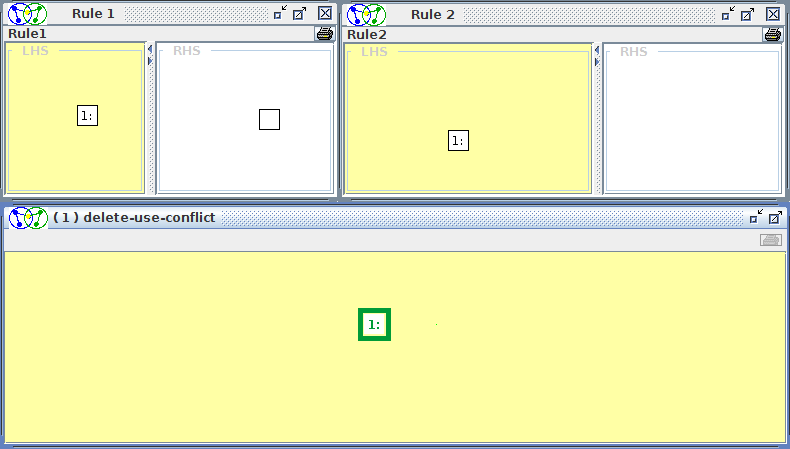
\includegraphics[width=\textwidth]{du}
\end{figure}

\end{frame}
%%%%%%%%%%%%%%%%%%%%%%%%

%%%%%%%%%%%%%%%%%%%%%%%%
\begin{frame}[fragile]{Delete-Use}{}

\centerline{
\xymatrix{
& & N_1 & & N_2 & & \\
R_1 & K_1\ar[d]_{k_1}\ar[l]_{r_1}\ar[r]^{l_1} & L_1\ar[dr]_{m_1}\ar[u]^{n_1} & \ar@{}[d] | >>*{\smallfrown}  & L_2\ar@{.>}@/_1.1pc/[dlll]_<<<<<<{!_{h_{21}}}\ar[dl]^{m_2}\ar[u]^{n_2} & K_2\ar[l]_{l_2}\ar[r]^{r_2} & R_2\\
 & D_1\ar[rr]_{d_1} & & G & & &}}

\vspace{1cm}

There is not exists $h_{21}:L_2 \rightarrow D_1 : d_1 \circ h_{21} = m_2$ and $\left(m_1,m_2\right)$ jointly surjective.

\end{frame}
%%%%%%%%%%%%%%%%%%%%%%%%

%%%%%%%%%%%%%%%%%%%%%%%%
\begin{frame}[fragile]{Delete-Use}{}

\color{blue}
\footnotesize
\begin{haskell}
allDeleteUse :: (EpiPairs m, DPO m) =>
  Bool -> Bool -> Production m -> Production m -> [CriticalPair m]
allDeleteUse nacInj inj l r =
 map (\match -> CriticalPair match Nothing Nothing DeleteUse) delUse
  where
    pairs = createPairsCodomain inj (left l) (left r)
    gluing = filter (\(m1,m2) -> satsGluingNacs nacInj inj (l,m1) (r,m2)) pairs
    delUse = filter (deleteUse inj l) gluing

deleteUse :: DPO m => Bool -> Production m -> (m, m) -> Bool
deleteUse inj l (m1,m2) = null matchD
  where
    (_,d1) = RW.poc m1 (left l)
    l2TOd1 = matches (flagInj inj) (domain m2) (domain d1)
    matchD = filter (\x -> m2 == compose x d1) l2TOd1
\end{haskell}
\color{black}

\end{frame}
%%%%%%%%%%%%%%%%%%%%%%%%

%%%%%%%%%%%%%%%%%%%%%%%%
\begin{frame}{Produce-Dangling Example}{}

\begin{figure}
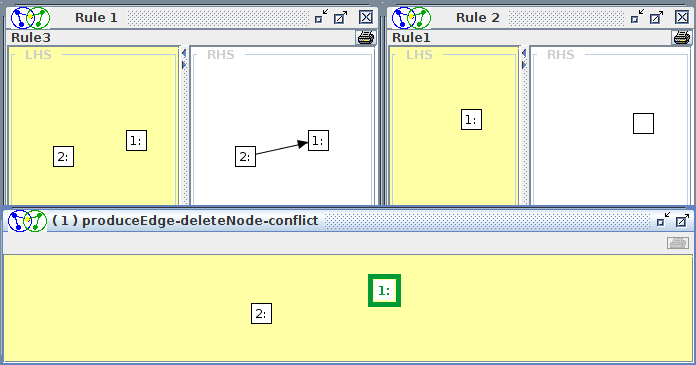
\includegraphics[width=\textwidth]{pd}
\end{figure}

\end{frame}
%%%%%%%%%%%%%%%%%%%%%%%%

%%%%%%%%%%%%%%%%%%%%%%%%
\begin{frame}[fragile]{Produce-Dangling}{}

\footnotesize
\centerline{
\xymatrix{
& & N_1 & & N_2 & & \\
R_1\ar[d]_{m_1'} & K_1\ar[d]^{k_1}\ar[l]_{r_1}\ar[r]^{l_1} & L_1\ar[dr]_{m_1}\ar[u]^{n_1} & \ar@{}[d] | >>*{\smallfrown} & L_2\ar@/_1.1pc/[dlll]_<<<<<<{h_{21}}\ar@/_2.5pc/[dllll]_<<<<<{he_{21}}\ar[dl]^{m_2}\ar[u]^{n_2} & K_2\ar[l]_{l_2}\ar[r]^{r_2} & R_2\\
P_1 & D_1\ar[l]^{e_1}\ar[rr]_{d_1} & & G & & &}}

\begin{figure}[h]
  \begin{minipage}{0.55\linewidth}
   There exists $h_{21}: L_2 \rightarrow D_1 : d_1 \circ h_{21} = m_2$ and $he_{21} : L_2 \rightarrow P_1 : h_{21} \circ e_1 = he_{21}$, let (1) the \emph{initial pushout} of $he_{21}$, there is not exists $b_2^* : B_2 \rightarrow K_2 : l_2 \circ b_2^* = b_2$, and $\left(m_1,m_2\right)$ jointly surjective.
  \vspace{4ex}
  \end{minipage}
  \hspace{0.1\linewidth}
  \begin{minipage}{0.35\linewidth}
    \centering
    \xymatrix{
B_2\ar[r]^{b_2}\ar[d]\ar@{.>}@/^1.5pc/[rr]^{!_{b_2^*}}\ar@{}[dr]|{(1)} & L_2\ar[d]^{he_{21}} & K_2\ar[l]_{l_2}\\
C_2\ar[r] & P_1 &}
  \vspace{4ex}
  \end{minipage}
\end{figure}

\end{frame}
%%%%%%%%%%%%%%%%%%%%%%%%

%%%%%%%%%%%%%%%%%%%%%%%%
\begin{frame}{Produce-Forbid Example}{}

\begin{figure}
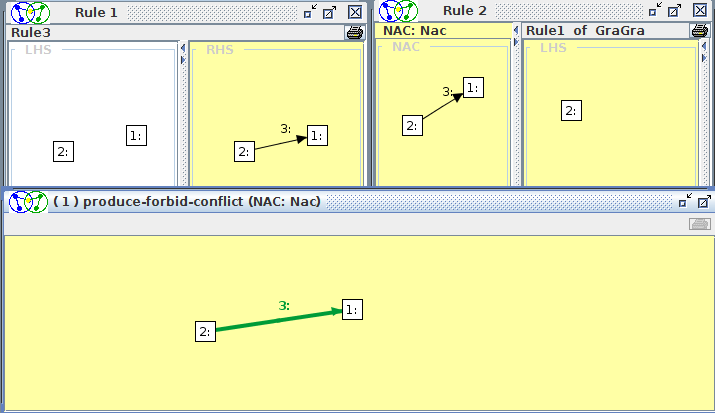
\includegraphics[width=\textwidth]{pf}
\end{figure}

\end{frame}
%%%%%%%%%%%%%%%%%%%%%%%%

%%%%%%%%%%%%%%%%%%%%%%%%
\begin{frame}[fragile]{Produce-Forbid}{}

\footnotesize
\centerline{
\xymatrix{
&  \ar@{}[ddl] | >>>*{\smallfrown\text{ }} & N_1 & & N_2\ar@/_2pc/[ddllll]_>>>>>>>>>>>>>>>{q21} & & \\
R_1\ar[d]_<<<<{m_1'} & K_1\ar[d]_<<<<{k_1}\ar[l]_{r_1}\ar[r]^{l_1} & L_1\ar[dr]_{m_1}\ar[u]_{n_1} & & L_2\ar@/_1.1pc/[dlll]_<<<<<<{h_{21}}\ar[dl]^{m_2}\ar[u]^{n_2} & K_2\ar[l]_{l_2}\ar[r]^{r_2} & R_2\\
P_1 & D_1\ar[l]^{e_1}\ar[rr]_{d_1} & & G & & &}}

\vspace{1cm}

There exists $h_{21}: L_2 \rightarrow D_1 : d_1 \circ h_{21} = m_2$ but for one of the NACs $n_2 : L_2 \rightarrow N_2$ of $p_2$ there exists an injective morphism $q_{21} : N_2 \rightarrow P_1 : q_{21} \circ n_2 = e_1 \circ h_{21}$ and thus, $e_1 \circ h_{21} \nvDash n_2$, and $\left(m'_1,q_{21}\right)$ jointly surjective.

\end{frame}
%%%%%%%%%%%%%%%%%%%%%%%%

%%%%%%%%%%%%%%%%%%%%%%%%
\begin{frame}{Critical Sequences}{}

\bi
\tm Same algorithm of Critical Pairs
\tm Inverts left rule
\tm Shift all nacs
\tm \footnotesize
\centerline{
\xymatrix{
& & N_1' & & N_2 & & \\
L_1\ar[d]_<<<<{m_1} & K_1\ar[d]\ar[l]_{l_1}\ar[r]^{r_1} & R_1\ar[dr]_{m_1'}\ar[u]_{n_1'} & \ar@{}[d] | >>*{\smallfrown} & L_2\ar[dl]^{m_2'}\ar[u]^{n_2} & K_2\ar[l]_{l_2}\ar[r]^{r_2} & R_2\\
G & D_1\ar[l]\ar[rr] & & P & & &}}
\ei

\end{frame}
%%%%%%%%%%%%%%%%%%%%%%%%

%%%%%%%%%%%%%%%%%%%%%%%%
\begin{frame}[fragile]{Implemented Algorithms}{}

\bi
\tm Concurrent Rules:
\begin{itemize}
\item $n = 0$ The \emph{concurrent rule} $p_c$ with NACs for rule $p_0$ with NACs is $p_0$ with NACs itself.
\item $n \geqslant 1$ A concurrent rule $p_c = p'_c \ast_E p_n $ with NACs for the rule sequence \rulesequence is defined recursively as $p_c = (l_c \circ k_c : K \rightarrow L, r_n \circ k_n : K \rightarrow R)$
\end{itemize}
\centerline{
\xymatrix{
  N_i & & & & N_j & & \\
  L'_c\ar[d]_{l'}\ar[u]^{n_i}\ar@{}[dr]|{(3)} & K'_c\ar[d]\ar[l]\ar[r] \ar@{}[dr]|{(1)} & R'_c\ar[dr]^{e_1} & \ar@{}[d] | >>*{\smallfrown} & L_n\ar[dl]_{e_2}\ar[u]^{n_j} & K_n\ar[d]\ar[l]\ar[r]\ar@{}[dl]|{(2)} & R_n\ar[d]\ar@{}[dl]|{(4)}\\
  L & C_c\ar[l]^{l_c}\ar[rr]_{r_c} & & \textit{E} & & C_n\ar[ll]^{l_n}\ar[r]_{r_n} & R\\
  & & & K\ar@{.>}@/1pc/[llu]^{k_c}\ar@{.>}@/1pc/[urr]_{k_n}\ar@{}[u]|{(5)} & & & 
}}
\ei
\end{frame}

\begin{frame}[fragile]{Implemented Algorithms}{}
\begin{haskell}
concurrentRuleForPair :: (DPO m, EpiPairs m, Eq (Obj m)) => Bool -> Production m -> Production m -> (m, m) -> Production m
concurrentRuleForPair inj c n pair = production l r (dmc ++ lp)
  where
    pocC = poc (fst pair) (right c)
    pocN = poc (snd pair) (left n)
    poC = po (fst pocC) (left c)
    poN = po (fst pocN) (right n)
    pb = injectivePullback (snd pocC) (snd pocN)
    l = compose (fst pb) (snd poC)
    r = compose (snd pb) (snd poN)
    dmc = concatMap (downwardShift inj (fst poC)) (nacs c)
    inverseP = production (snd pocC) (snd poC) []
    den = concatMap (downwardShift inj (snd pair)) (nacs n)
    lp = concatMap (shiftLeftNac inj inverseP) den
\end{haskell}
\end{frame}

\iffalse
\begin{frame}[fragile]{Implemented Algorithms}{}

\bi 
\tm Concurrent Rules:
\begin{itemize}
\item $n = 0$ The \emph{concurrent rule} $p_c$ with NACs for rule $p_0$ with NACs is $p_0$ with NACs itself.
\item $n \geqslant 1$ A concurrent rule $p_c = p'_c \ast_E p_n $ with NACs for the rule sequence \rulesequence is defined recursively as $p_c = (l_c \circ k_c : K \rightarrow L, r_n \circ k_n : K \rightarrow R)$ where 
  \begin{itemize}
  \item $p'_c : L'_c \leftarrow K'_c \rightarrow R'_c$ is a concurrent rule for the sequence $p_0,\ldots,p_{n-1}$
  \item $(e'_c,e_n)$ is jointly surjective
  \item (1), (2), (3) and (4) are pushouts
  \item (5) is a pullback
  \item $N_i$ is shifted over morphism $l'$
  \item $N_j$ is shifted over morphism $e_2$ and then over the ``rule'' $q'_c = l_c : C_c \rightarrow L, r_c : C_c \rightarrow E$
  \end{itemize}
\end{itemize}
\ei
\end{frame}
\fi
\begin{frame}[fragile]{Implemented Algorithms}{}

\bi
\tm NAC shifted over a morphism:
\centerline{\xymatrix{
  N'_j\ar@{.>}@/0.5pc/[r]^{e_{ji}} & N_i\ar@{}[dl]|{=}\\
  A\ar[r]_{m}\ar[u]^{n'_j} & B\ar[u]_{n_i}
}}

For each $NAC(n'_j)$ on $A$ with $n'_j : A \rightarrow N'_j$ and $m : A \rightarrow B$, let 

\begin{center}
$D_m(NAC(n'_j)) = \{ NAC(n_i)|i \in I, n_i : B \rightarrow N_i \}$
\end{center}

where $I$ and $n_i$ are constructed as follows:

\begin{itemize}
\item $i \in I$ iff $(e_{ji}, n_i)$ with $e_{ji} : N'_j \rightarrow N_i$ jointly surjective 
\item $e_{ji} \circ n_i = n_i \circ m$
\item $e_{ji}$ injective
\end{itemize}
\ei

\end{frame}

\begin{frame}[fragile]{Implemented Algorithms}{}

\bi
\tm NAC shifted over a morphism:
\\
\begin{haskell}
downwardShift :: EpiPairs m => Bool -> m -> m -> [m]
downwardShift inj m n = newNacs
  where
    pairs = commutingPairsAlt (n,True) (m,inj)
    newNacs = map snd pairs
\end{haskell}
\ei
\end{frame}


\begin{frame}[fragile]{Implemented Algorithms}{}

\bi
\tm Left NACs from Right NACs

For each $NAC(n_i)$ on $R$ of a rule, the equivalent left application condition $L_p(NAC(n_i))$ is defined in the following way:

\centerline{\xymatrix{
  L\ar[d]_{n'_i} & K\ar[l]\ar[r]\ar[d] & R\ar[d]^{n_i}\\
  N'_i\ar@{}[ur]|{(2)} & D\ar[l]\ar[r] & N_i\ar@{}[ul]|{(1)}
}}

\begin{itemize}
\item If the pair $(K \rightarrow R, R \rightarrow N_i)$ has a pushout complement, we construct $(K \rightarrow D, D \rightarrow N_i)$ as the pushout complement (1). Then we construct pushout (2) with the morphism $n'_i : L \rightarrow N'_i$.
\item If the pair $(K \rightarrow R, R \rightarrow N_i)$ does not have a pushout complement, we define $L_p(NAC(n_i)) = true$
\end{itemize}
\ei

\begin{haskell}
shiftLeftNac inj rule n = [comatch n rule | satsGluing inj n (left rule)]
\end{haskell}

\end{frame}





%%%%%%%%%%%%%%%%%%%%%%%%

%%%%%%%%%%%%%%%%%%%%%%%%
\begin{frame}[fragile]{Interlevel Conflicts}{}

\centerline{
\xymatrix@R=0.3cm@C=0.3cm{
a_3\ar[ddd]|{m_3} &&& b_3\ar[lll]\ar[rrr]\ar[ddd] &&& c_3\ar[ddd] \\
& a_2\ar[ul]\ar[ddd]|{m_2}\ar[dr] &&& b_2\ar[ul]\ar[lll]\ar[rrr]\ar[dr]\ar[ddd] &&& c_2\ar[ul]\ar[dr]\ar[ddd] \\
&& a_1\ar[ddd]|{m_1} &&& b_1\ar[lll]\ar[rrr]\ar[ddd] &&& c_1\ar[ddd] \\
R\ar[ddd] &&& R'\ar[lll]\ar[rrr] &&& R'' \\
& K\ar[ul]|{r}\ar[ddd]\ar[dr]|{l} &&& K'\ar[ul]\ar[lll]\ar[rrr]\ar[dr] &&& K''\ar[ul]|{r''}\ar[dr]|{l''} \\
&& L\ar[ddd]|{m_0} &&& L'\ar[lll]|{f_L}\ar[rrr]|{g_L} &&& L''\ar[dddllllll]|{m_0''} \\
H \\
& D\ar[ul]\ar[dr] \\
&& G}}

\end{frame}
%%%%%%%%%%%%%%%%%%%%%%%%

%%%%%%%%%%%%%%%%%%%%%%%%
\begin{frame}[fragile]{Interlevel Conflicts Examples}{}

\begin{figure}
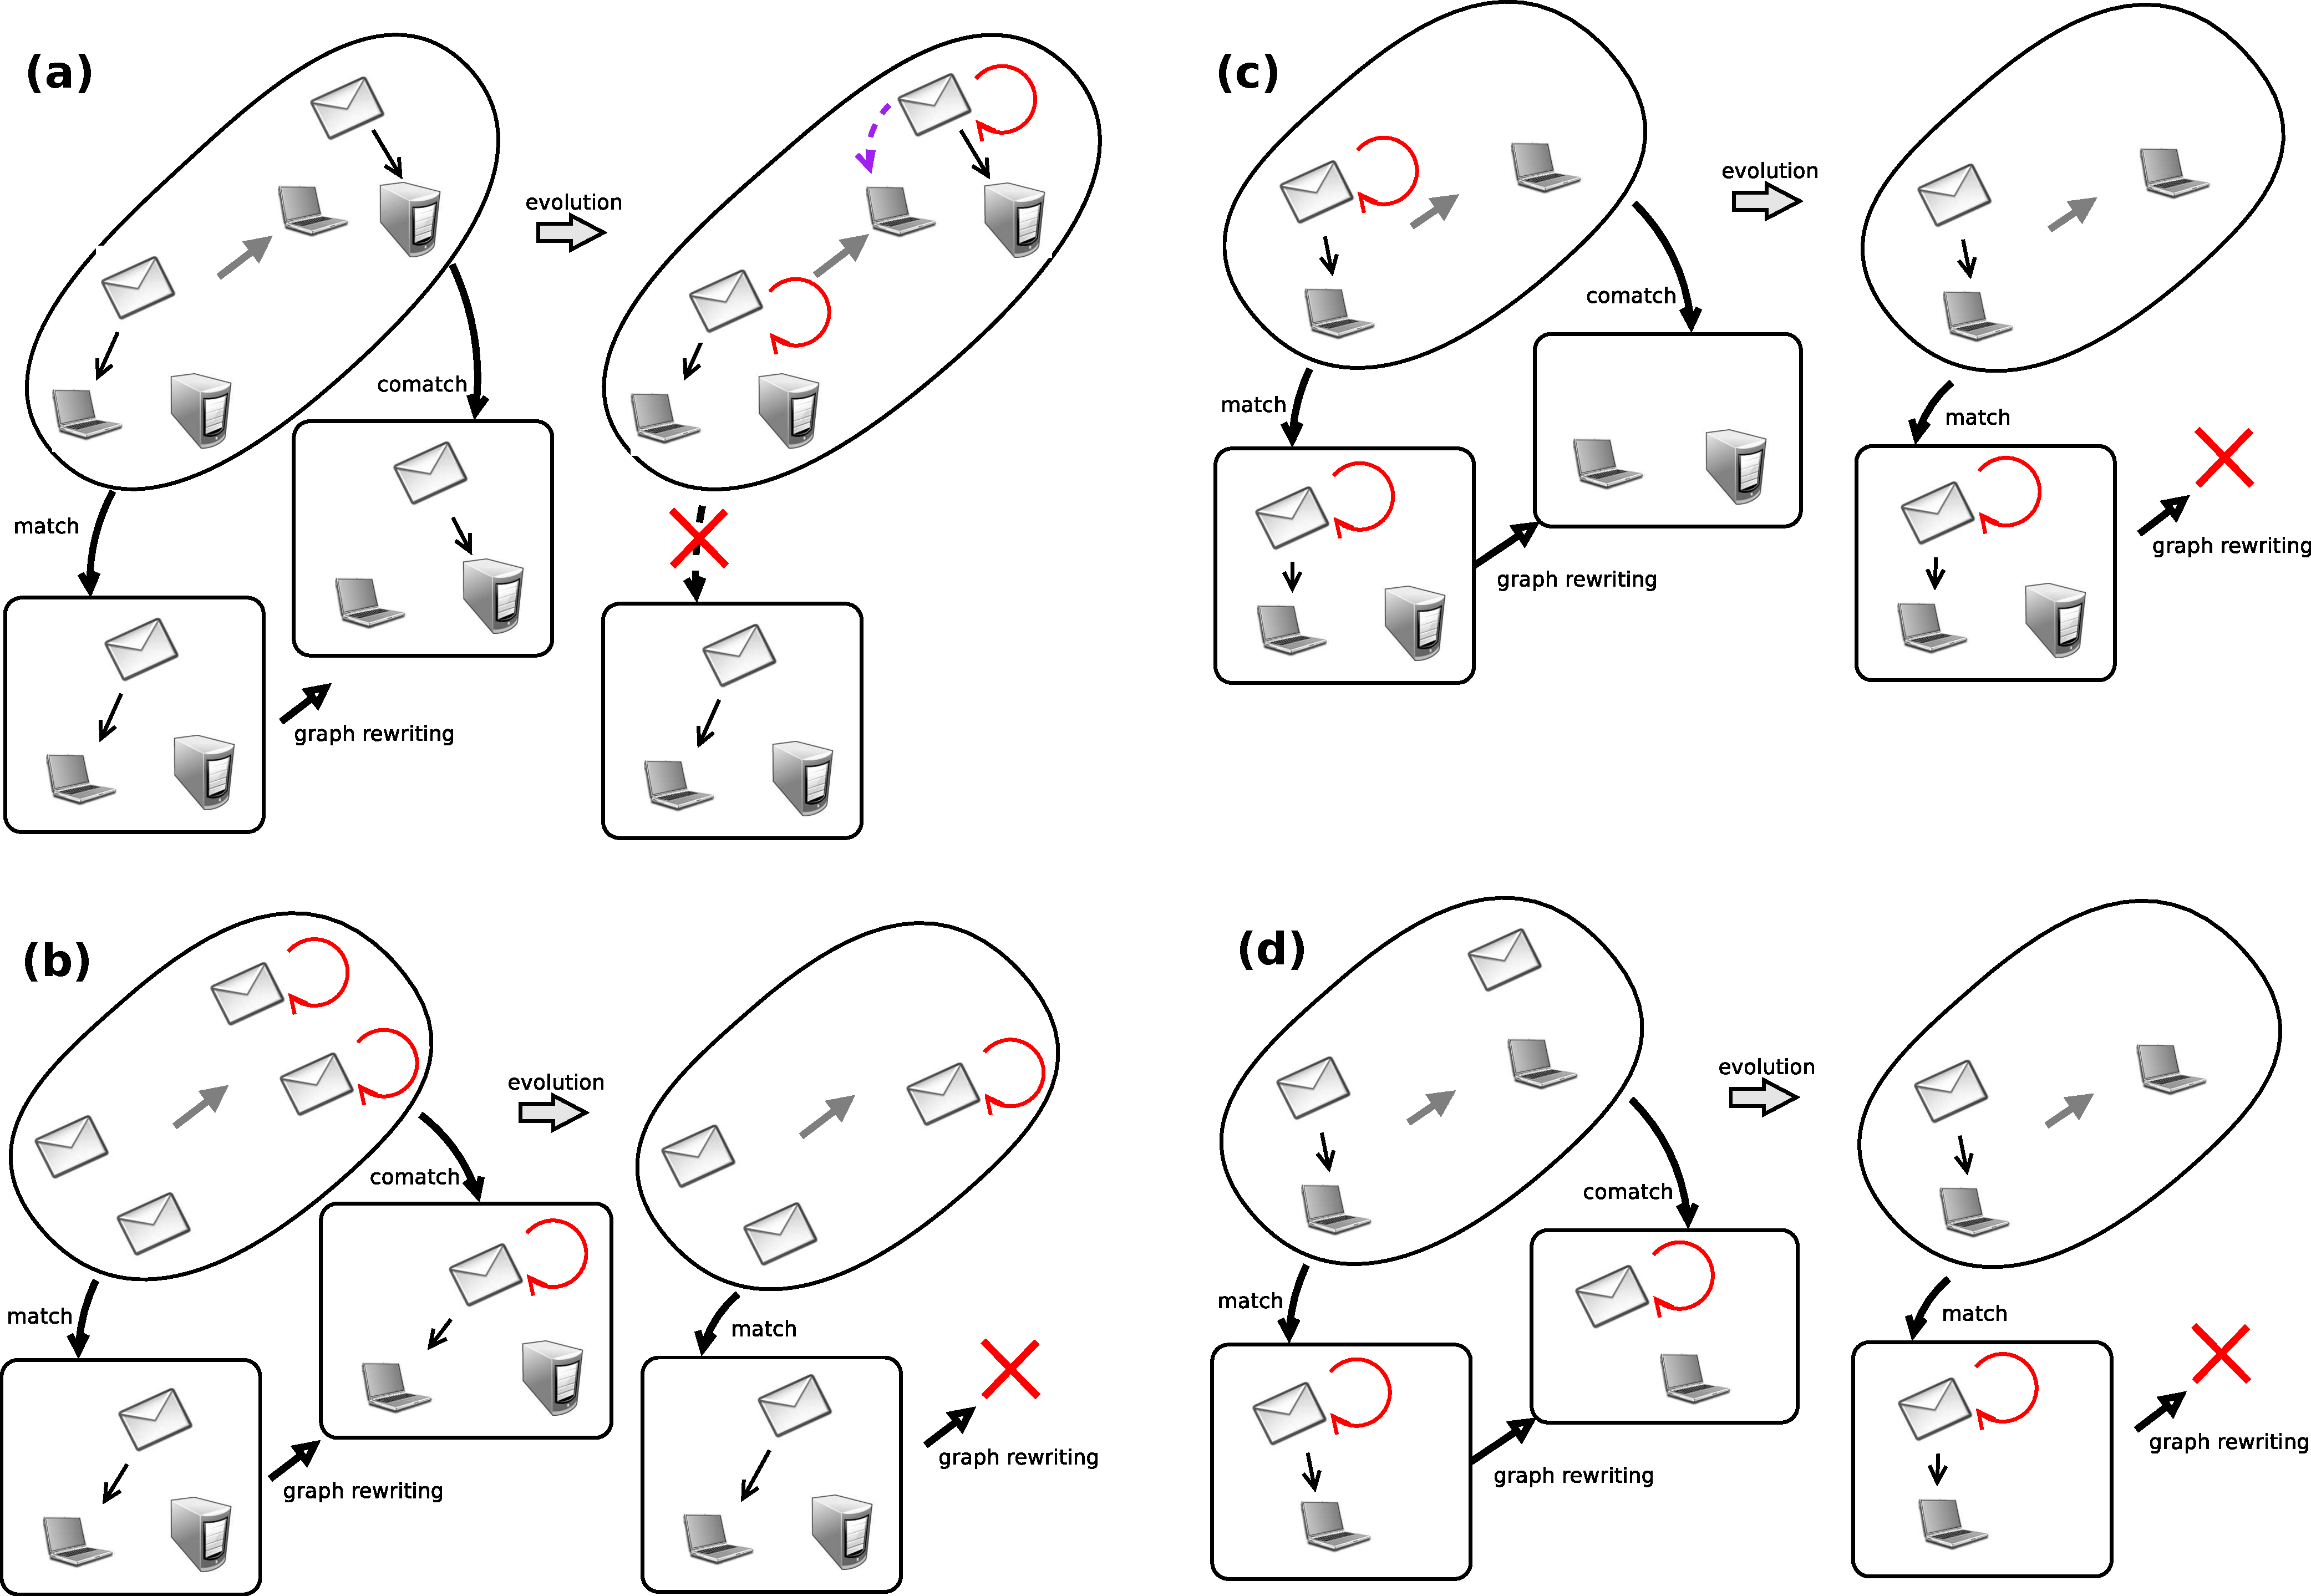
\includegraphics[width=0.95\textwidth]{example-conflict-03}
\end{figure}

\end{frame}
%%%%%%%%%%%%%%%%%%%%%%%%

\section{Usage}

%%%%%%%%%%%%%%%%%%%%%%%%
\begin{frame}{IO}{}

\bi
\tm AGG
\bi
\tm Input
\bi
\tm .ggx
\ei
\ei
\bi
\tm Output
\bi
\tm .cpx
\tm .ggx
\ei
\ei
\tm Haskell $Read$ and $Show$ 
\ei

\end{frame}
%%%%%%%%%%%%%%%%%%%%%%%%

%%%%%%%%%%%%%%%%%%%%%%%%
\begin{frame}{Usage}{}

\bi
\tm Commands
\bi
\tm analysis
\bi
\tm --snd-order
\tm --conflicts-only
\tm --dependencies-only
\ei
\tm concurrent-rule
\bi
\tm --max-rule
\tm --all-rules
\tm --by-dependency
\ei
\tm snd-order
\ei
\tm Options
\bi
\tm --all-matches
\tm --inj-nac-satisfaction
\ei
\ei

\end{frame}
%%%%%%%%%%%%%%%%%%%%%%%%

\section{Functionalities under study}

%%%%%%%%%%%%%%%%%%%%%%%%
\begin{frame}[fragile]{Functionalities under study}{}

\bi
\tm Attributed Graph Grammars
\bi
\tm DPO for the Category of Algebras
\tm Critical Pairs
\tm Concurrent Rules
\ei
\tm Second-order with non-injective matches
\tm Improvement of inter level CP algorithm
\ei

\end{frame}
%%%%%%%%%%%%%%%%%%%%%%%%

\section{Future Work}

%%%%%%%%%%%%%%%%%%%%%%%%
\begin{frame}[fragile]{Future Work}{}

\bi
\tm Graphical User Interface
\tm Initial Pushout and Critical Objects
\tm Inheritance
\tm AGREE
\ei

\end{frame}
%%%%%%%%%%%%%%%%%%%%%%%%

\end{document}
